\documentclass[BTech]{iitmdiss}

\usepackage{lmodern}
\usepackage[scaled=0.8]{beramono}
\usepackage{t1enc}

\usepackage{graphicx}
\usepackage{epstopdf}
\usepackage[hypertex]{hyperref}
\usepackage{amsmath}
\usepackage{amssymb}
\usepackage{fancyvrb}
\usepackage[ruled,lined,commentsnumbered]{algorithm2e}
\usepackage{color}
\usepackage{listings}

\VerbatimFootnotes
\graphicspath{ {./images/} }

\captionsetup{font=footnotesize}

\definecolor{mygreen}{rgb}{0,0.6,0}
\definecolor{mygray}{rgb}{0.5,0.5,0.5}
\definecolor{mymauve}{rgb}{0.58,0,0.82}
\lstset{
	backgroundcolor=,                      % choose the background color; you must add \usepackage{color} or \usepackage{xcolor}
	basicstyle=\ttfamily,                  % the size of the fonts that are used for the code
	breakatwhitespace=false,               % sets if automatic breaks should only happen at whitespace
	breaklines=true,                       % sets automatic line breaking
	captionpos=b,                          % sets the caption-position to bottom
	commentstyle=\itshape\color{mygreen},  % comment style
	frame=L,                               % adds a frame around the code
	keepspaces=true,                       % keeps spaces in text, useful for keeping indentation of code (possibly needs columns=flexible)
	keywordstyle=\color{blue},             % keyword style
	language=C++,                          % the language of the code
	numbers=left,                          % where to put the line-numbers; possible values are (none, left, right)
	numbersep=10pt,                        % how far the line-numbers are from the code
	numberstyle=\tiny\color{mygray},       % the style that is used for the line-numbers
	rulecolor=\color{black},               % if not set, the frame-color may be changed on line-breaks within not-black text (e.g. comments (green here))
	showspaces=false,                      % show spaces everywhere adding particular underscores; it overrides 'showstringspaces'
	showstringspaces=false,                % underline spaces within strings only
	showtabs=false,                        % show tabs within strings adding particular underscores
	stepnumber=2,                          % the step between two line-numbers. If it's 1, each line will be numbered
	stringstyle=\color{mymauve},           % string literal style
	tabsize=4,                             % sets default tabsize to 2 spaces
	title=\lstname,                        % show the filename of files included with \lstinputlisting; also try caption instead of title
	xleftmargin=\parindent
}

% For the underbar vector notation, without losing the italics
\newcommand{\ue}[1]{\underbar{\emph{#1}}}

% For aligning subscripts and superscripts in correlation expressions
\newcommand{\corr}[2]{#1^{} #2^*}

% For inserting a blank page
\newcommand{\blankpage}[0]{
  \newpage
  \null
  \thispagestyle{empty}
  \newpage
}


\begin{document}

\title{A MODULARIZED OFDM STACK \\
       FOR COMMUNICATION USING \\
       UNIVERSAL SOFTWARE DEFINED \\
       RADIO PERIPHERALS}

\author{PRAVEEN VENKATESH}

\date{JUNE 2014}
\department{ELECTRICAL ENGINEERING}

\maketitle

\certificate

\vspace*{0.5in}

\noindent This is to certify that the thesis titled {\bf A Modularized OFDM
Stack for Communication using Universal Software Defined Radio Peripherals},
submitted by {\bf Praveen Venkatesh}, to the Indian Institute of Technology,
Madras, in partial fulfillment of the requirements for the award of the degree
of {\bf Bachelor of Technology}, is a bona fide record of the work done by him
under our supervision. The contents of this thesis, in full or in parts, have
not been submitted to any other Institute or University for the award of any
degree or diploma.

\vspace*{1.5in}

\begin{singlespacing}
\hspace*{-0.25in}
\parbox{2.5in}{
	\noindent {\bf Prof.~Radhakrishna~Ganti} \\
	\noindent Research Guide \\
	\noindent Assistant Professor \\
	\noindent Dept. of Electrical Engineering\\
	\noindent IIT Madras - 600 036 \\
}
\hspace*{1.0in}
\end{singlespacing}

\vspace*{0.25in}

\noindent Place: Chennai \\
Date: 13 June, 2014

\acknowledgements

I'd sincerely like to thank my guide, Prof.\ Radhakrishna Ganti, for always
being there whenever I had a problem. I don't think I could have asked for
anything more in a guide, considering how he's physically sat alongside me,
reading obscure code and helping me figure out the problems.

Second, I'd like to thank Arjun for helping me through this entire journey. He,
too, has always been there when I needed someone to bounce ideas off, to check
my code, or otherwise help me figure out some problem.

I'd like to thank Prof.\ HSR for giving me some useful advice when I needed it,
and for being supportive when I chose to make the switch to Comm. I'd also like
to thank the other members of my lab, for making it a pleasant (if, at times,
somewhat PJ-filled) working environment.

Last, but not the least, I'd like to thank my family for giving me the freedom
to choose anyhow I wished, and for being fully supportive of any decision I
took.

\abstract

\noindent \textsc{keywords} \hspace*{0.5em} \parbox[t]{4.4in} {Orthogonal
Frequency Division Multiplexing; Timing Synchronization; Universal Software
Defined Radio Peripheral; Log Likelihood Ratio, Joint Trellis Shaping; Dirty
Paper Coding}

\vspace*{24pt}

\noindent This report outlines the theory behind, the working of, and the
design decisions that went into the creation of an OFDM stack and a few other
modules that were constructed primarily as component blocks of a larger
project aimed at implementing and demonstrating a real-time Dirty Paper Coding
framework in a base-station-with-two-users environment. The report aims to be
used as a reference design document for future generations of this framework.

\pagebreak
\begin{singlespace}
\tableofcontents
\thispagestyle{empty}

\listoftables
\addcontentsline{toc}{chapter}{LIST OF TABLES}
\listoffigures
\addcontentsline{toc}{chapter}{LIST OF FIGURES}
\end{singlespace}

\abbreviations

\noindent
\begin{tabbing}
	xxxxxxxxxxx \= xxxxxxxxxxxxxxxxxxxxxxxxxxxxxxxxxxxxxxxxxxxxxxxx \kill
	\textsc{ofdm} \> Orthogonal Frequency Division Multiplexing \\
	\textsc{usrp} \> Universal Software Defined Radio Peripheral \\
	\textsc{isi}  \> Inter-Symbol Interference \\
	\textsc{llr}  \> Log-Likelihood Ratio \\
	\textsc{qam}  \> Quadrature Amplitude Modulation \\
	\textsc{dpc}  \> Dirty Paper Coding \\
	\textsc{ldpc} \> Low Density Parity Check (code) \\
\end{tabbing}

\pagebreak

%%%%%%%%%%%%%%%%%%%%%%%%%%%%%%%%%%%%%%%%%%%%%%%%%%%%%%%%%%%%%%%%%%%%%%%%%%%%%%%

\clearpage

% The main text will follow from this point so set the page numbering
% to arabic from here on.
\pagenumbering{arabic}

%%%%%%%%%%%%%%%%%%%%%%%%%%%%%%%%%%%%%%%%%%%%%%%%%%%%%%%%%%%%%%%%%%%%%%%%%%%%%%%
% Chapters

\chapter{INTRODUCTION}
\label{chap:intro}

\section{Orthogonal Frequency Division \\ Multiplexing}

\subsection{Digital communication}

When transmitting digital data over a real (analog) channel, we typically first
convert the bit stream into a stream of complex symbols, using some kind of
modulation scheme. Following this, the symbols are pulse-shaped and upconverted
to the carrier frequency, real and imaginary parts of the symbols being encoded
in the in-phase and quadrature components of the carrier.

We can retrieve the complex symbols on the receiver side by performing matched
filtering followed by suitably sampling the analog data. In such a scenario,
the effects of the channel can also be viewed as purely digital operations on
the complex data stream. We can, therefore, work at the level of digital
abstraction, where we only deal with a discrete sequence of complex symbols.

\subsection{Channel effects}

The modulation scheme used will decide how robust the message will be against
channel effects. A simple but effective digital channel model has an impulse
response to model inter-symbol interference (caused due to multi-path effects
in wireless transmission, for example) and an addition of white gaussian noise.
Simple modulation schemes such as QAM do not fare well in such a channel,
however, due to ISI.

In order combat the effect of ISI in such cases, we would need to employ
computationally intensive decoding techniques such as the Viterbi algorithm.
Alternatives are to use sub-optimal equalization filters such as the
zero-forcing equalizer, but depending upon how many taps the channel has, these
filters could turn out to be extremely long, which once again, makes them
computationally intensive.

\subsection{OFDM solves the ISI problem}

OFDM is a modulation scheme that effectively solves the problem of ISI without
introducing heavy computational complexity. It does this by placing a block of
complex data symbols on adjacent narrow-band `subcarriers' in the frequency
domain. The transmitted data block is the inverse-FFT of the frequency domain
block. On the receiver side, each data block is converted back into frequency
domain by taking the FFT of the block.

Each block of data, after the inverse-FFT is performed, is prepended with a
cyclic prefix, which is a copy of the last few symbols. The length of this
cyclic prefix is equal to the number of taps in the channel's impulse response.
The cyclic prefix ensures that the effects of ISI remain limited to the same
data block and guards against pollution of symbols from adjacent data blocks.

With this framework, the ISI of the channel gets expressed in frequency domain
as frequency-selective fading, with each subcarrier seeing a different gain.
If we have a model of the channel in frequency domain, (by taking the FFT of
the channel taps), then we can reverse the effects of ISI completely by simply
dividing each received subcarrier symbol by the channel response at that
subcarrier.

\cite{py:python}

\chapter{TIMING ANALYSIS}
\label{chap:timing}

%%%%%%%%%%%%%%%%%%%%%%%%%%%%%%%%%%%%%%%%%%%%%%%%%%%%%%%%%%%%%%%%%%%%%%%%%%%%%%%

\section{Packet detection}

Timing analysis is used to determine the point in time where the packet starts.
This is also a method to recognize \emph{whether} a packet has arrived or not.
In the current scheme, the packet detection module uses the Schmidl and Cox %(TODO: Put citation here)
method for timing analysis.

This entire section will assume a level of abstraction wherein we have an
inexhaustible data source of digital, complex symbols at the receiver. We
acquire this data by reading from this source into a buffer (which is simply an
array) in our receiver program's source code.

\subsection{The Schmidl and Cox algorithm}

For the receiver to be able to pick out a packet from ambient noise and
interference, the transmitted packet must be designed for detection. All
transmitted packets have a \emph{preamble}, which consists of two identical
halves. Each half is a pseudo-random-number sequence. The correlation of each
half with with other (independent and hence uncorrelated) signals is expected
to be low. However, its correlation with the other half will be high. Moreover,
this property is well-maintained even when the preamble is passed through an
ISI channel with additive white gaussian noise.

In other words, we can detect the start of a packet by correlating two adjacent
windows, each having half the size of the preamble, with each other. The point
where this correlation value becomes high can be taken to be the start of the
packet.

\begin{figure}[h]
	\centering
	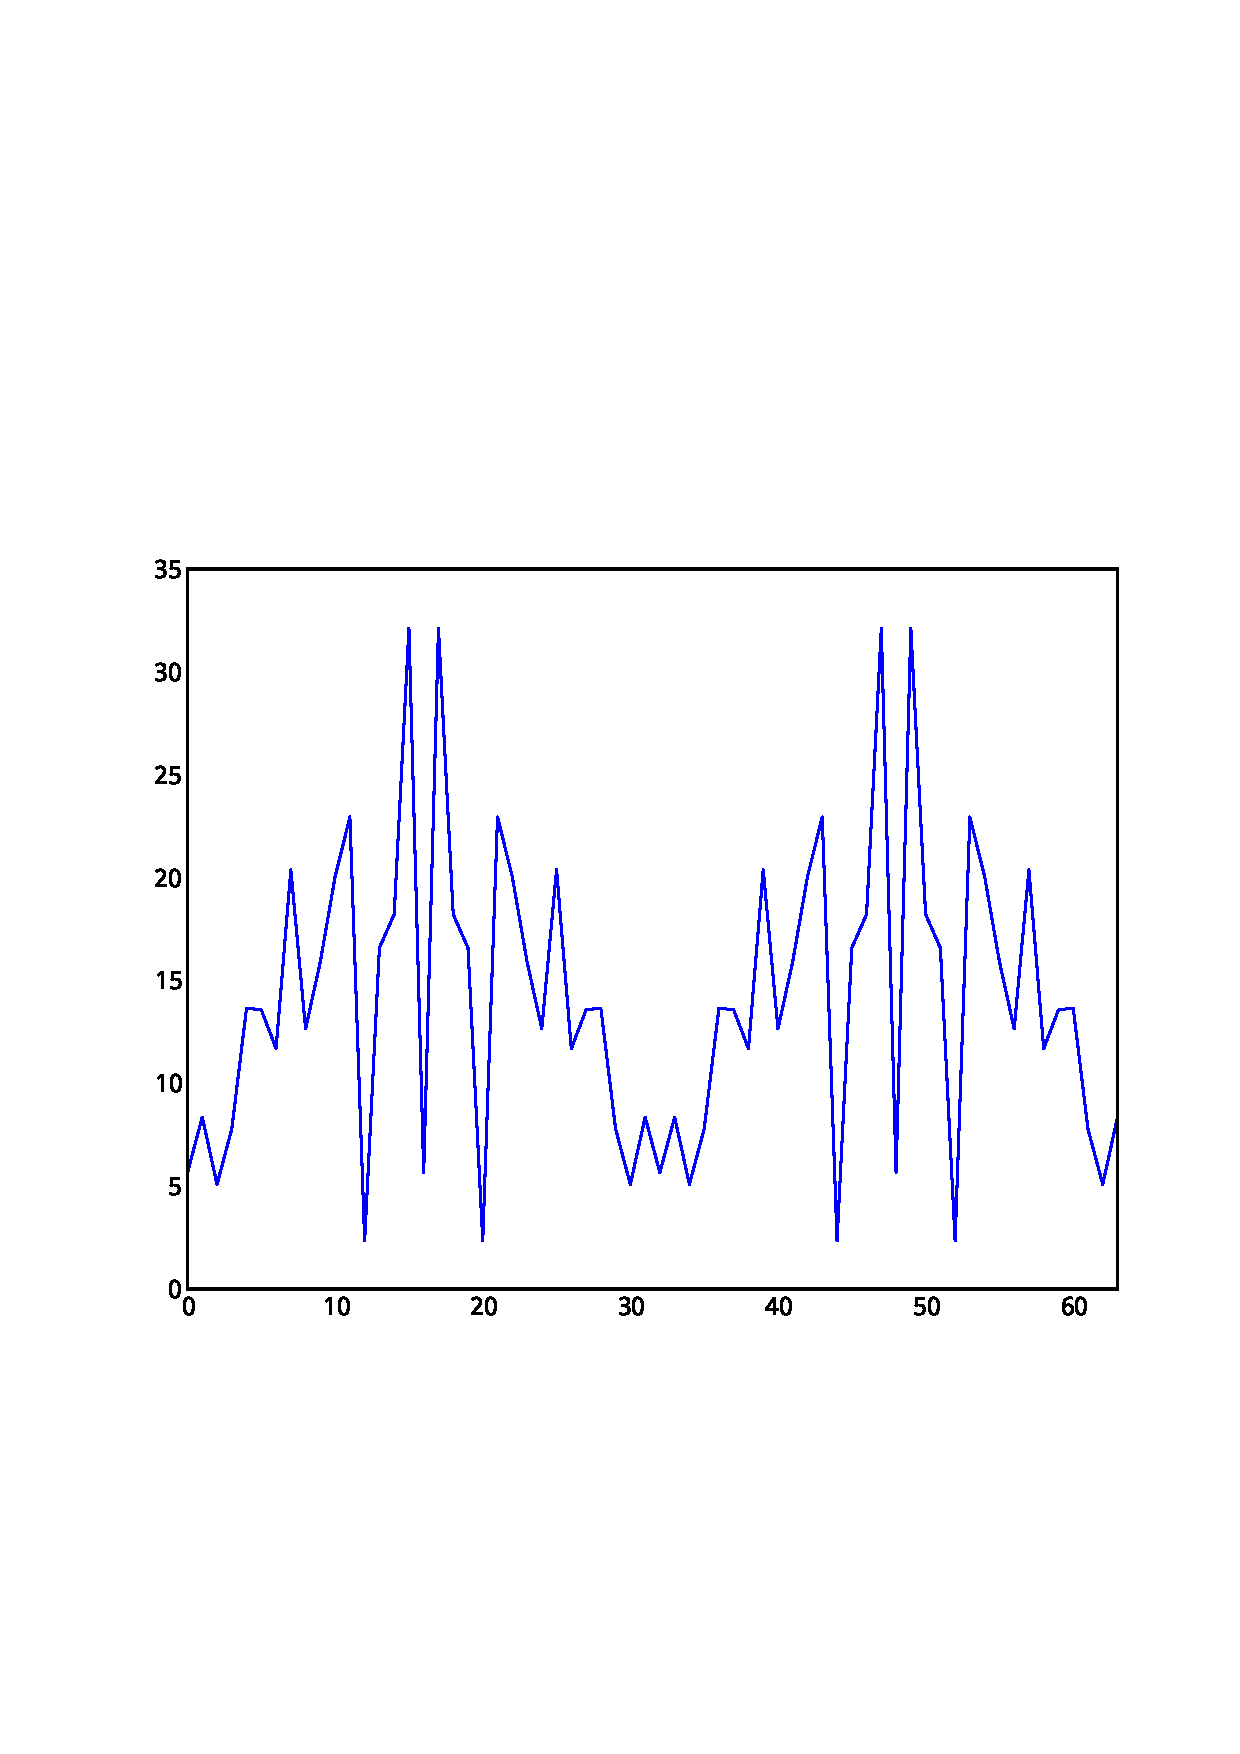
\includegraphics[width=0.8\textwidth]{preamble-abs}
	\caption{Absolute value of the preamble}
	\label{fig:preamble-abs}
\end{figure}

The metric used to determine whether or not the correlation value is high
enough is the normalized cross-correlation, defined as
$$ \text{Metric} = \frac{|\text{ Cross-correlation of the two windows }|}
                        {\sqrt\text{Product of the autocorrelations of the
                                    windows}}
$$
Let $\ue{x}$ be the vector of complex values corresponding to the first window
and $\ue{y}$ be that corresponding to the second. Then, the metric $m$ is
given by
\begin{equation} \label{eqn:old-metric}
	m = \frac{|\corr{\ue{x}}{\ue{y}}|}{|\ue{x}||\ue{y}|}
\end{equation}
where $(^*)$ denotes complex conjugation in the case of scalars and complex
conjugate transpose in the case of vectors. All vectors are taken to be row
vectors. A plot of this metric on actual transmitted data is shown in
figure~\ref{fig:metric}.

\begin{figure}[h]
	\centering
	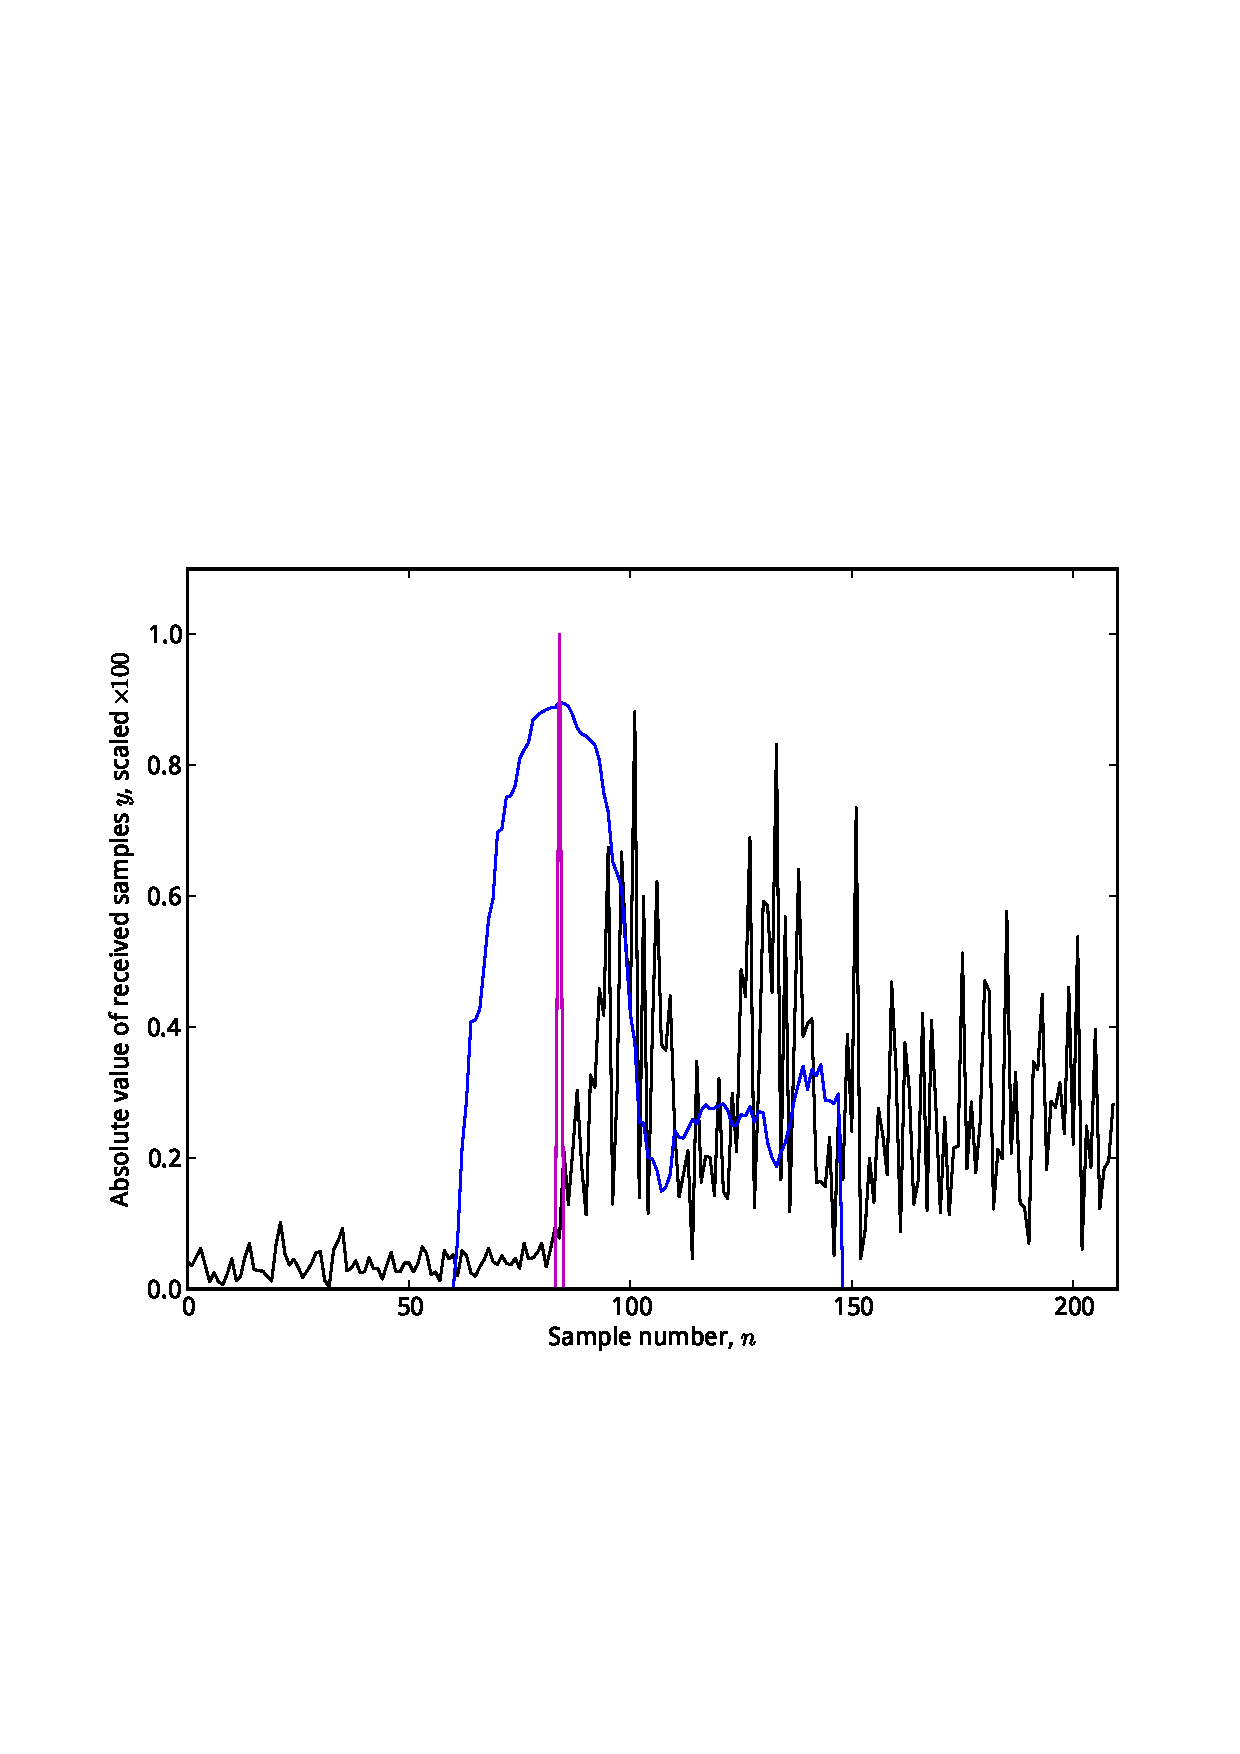
\includegraphics[width=0.8\textwidth]{metric}
	\caption{A sample plot of received data in black, with the metric overlayed
	         in blue. The sharp singular peak in magenta indicates the maximum
	         of the metric, which is taken to be the start of the preamble.
	         Note that the value of the metric is shown at the start of the two
	         correlation windows. Notice that although the channel distorts the
	         preamble, the two halves are still more or less identical. This is
	         the reason behind why this method of packet detection works. Also
	         notice how the metric stops soon after the peak is detected. The
	         reasoning behind this is explained in
	         subsection~\ref{subsec:stop-corr}.}
	\label{fig:metric}
\end{figure}

\subsection{Running correlation on the receive buffer}

In order to efficiently perform a running correlation of adjacent windows over
an entire receive buffer, we minimize the number of computations performed. On
moving one step, we add the latest correlation point and subtract the oldest
correlation point.

\begin{figure}[h]
	\centering
	
\includegraphics[width=0.8\textwidth]{correlation-windows}
	\caption{Correlation windows}
	\label{fig:corr-win}
\end{figure}

Let $\{x_i\}_{i=0}^{n-1}$ and $\{y_i\}_{i=0}^{n-1}$ be complex sequences
corresponding to the symbols in the left window and the right window
respectively, where $n$ is the window size, which is half the length of the
preamble. In the next time step, these windows are denoted as
$\{x_i\}_{i=1}^{n}$ and $\{y_i\}_{i=1}^{n}$ respectively.\footnote{Note that
for the purpose of these calculations, the two windows may be disconnected or
overlapping. No assumptions are made regarding the equality of certain ranges
of $x_i$ and $y_i$. Specifically, we do \emph{not} assume that $x_n = y_0$.
Thus, when $x_i = y_i\;\forall\;i\in\{0,1,\ldots n-1\}$, we automatically
arrive at the running \emph{auto}correlation formula.}

Let $c_{old}$ be the correlation of windows in the current time step, and
$c_{new}$ be the correlation of the windows in the next time step. That is,
\begin{equation}
	c_{old} = \sum_{i=0}^{n-1}{\corr{x_i}{y_i}}
\end{equation}
\begin{equation}
	c_{new} = \sum_{i=1}^n{\corr{x_i}{y_i}}
\end{equation}
We can then write $c_{new}$ in terms of $c_{old}$ as follows:
\begin{align}
	c_{new} &= \sum_{i=0}^{n-1}{\corr{x_i}{y_i}} - \corr{x_0}{y_0}
	                                             + \corr{x_n}{y_n} \\
	        &= c_{old} - \corr{x_0}{y_0} + \corr{x_n}{y_n}
	                                                     \label{eqn:old-update}
\end{align}

This way, once we have acquired the correlation of the first $n$ symbols, the
correlation of subsequent windows is an $\mathcal{O}(1)$ process.

\subsection{Implementation using the two-frame block}
\label{subsec:two-frame-impl}

In order to implement the Schmidl and Cox algorithm, we need to continuously
scan through the received symbols, correlating two windows, each half the size
of the preamble. Once the preamble is found, we need to pull out a full
\verb+frame_size+ number of symbols from the buffer.

Obviously, the receive buffer should be at least as long as the preamble. But
if the receive buffer is too long, then depending upon the rate of
communication, we may be adding latency to our program by having to wait for
the buffer to get filled. If our receive buffer is only one \verb+frame_size+
long, then on finding the preamble in the middle of this buffer, we will have
to take into account how many symbols more we need to extract for the frame
from the next buffer. This is cumbersome and error-prone.

\begin{figure}[h]
	\centering
	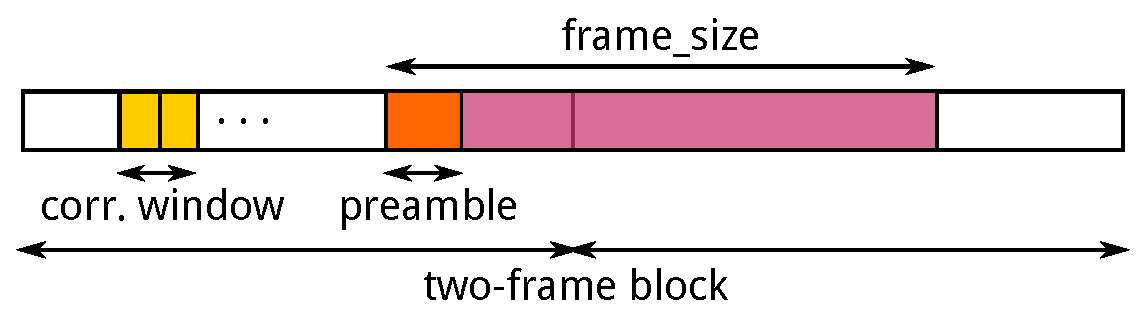
\includegraphics[width=0.8\textwidth]{two-frame-block}
	\caption{A depiction of the two-frame block used to buffer received complex
	         symbols}
	\label{fig:two-frame-block}
\end{figure}

A simpler implementation scheme involves having a receive buffer that is two
\verb+frame_size+s long. We refer to this buffer as the \emph{two-frame block}.
On each iteration, we search only the first half of the buffer. Even if the
preamble is found towards the end of the first half, we can still pull out a
full \verb+frame_size+ from the two-frame block.

%%%%%%%%%%%%%%%%%%%%%%%%%%%%%%%%%%%%%%%%%%%%%%%%%%%%%%%%%%%%%%%%%%%%%%%%%%%%%%%

\section{The DC offset problem}

The packet detection algorithm hinges on the fact that the only place where
the correlation yields a peak is when the two windows are identical. But when
there is a DC component present in the signal, the algorithm yields a high
correlation. We therefore need to eliminate the DC component in the signal
prior to performing the correlation.

\subsection{Discovering the DC offset}

We observed problems with packet detection, wherein received packets were not
getting decoded faithfully; there being no correlation between the transmitted
and received constellations. Upon plotting the start of the frame along with
the computed metric, we noticed the presence of two peaks of the metric (as
opposed to the expected one). The first peak, which was not caused by the
preamble, was being erroneously detected as the start of the frame, leading to
the rest of the frame being incorrectly decoded.

The reason for this was the presence of a large plateau prior to the start of
the preamble. This signal plateau constituted a DC signal, which correlates
positively with itself. Since the plateau was longer than the size of the two
correlation windows, we saw a metric peak at the start of the plateau.

%TODO: Put plots of the double-peak and plateau here.

\subsection{Eliminating the DC offset}

To stop a DC signal producing fake peaks in our metric, one option was to
correlate the signal with the preamble sequence itself (as described later in
subsection~\ref{subsec:fine-metric}). But this is a computationally expensive
proposition, since it is not possible to perform running correlations when one
of the vectors being run over is actually kept fixed.

We therefore eliminate the DC offset by subtracting out the mean of each window
before correlation. That is, instead of equation~\ref{eqn:old-metric}, we have
\begin{equation} \label{eqn:new-metric}
	m = \frac{|\corr{(\ue{x}-\bar{x})}{(\ue{y}-\bar{y})}|}
	         {|\ue{x}-\bar{x}||\ue{y}-\bar{y}|}
\end{equation}
where $\bar{x}$ refers to the mean of the vector $\ue{x}$.

This procedure has no effect on the preamble itself, since the pseudo random
noise sequence used for the preamble is zero-mean.

\subsection{Running correlations with DC offset elimination}

In order to perform running correlations with the new metric, we need to
come up with an update equation similar to equation~\ref{eqn:old-update}.

\begin{figure}[h]
	\centering
	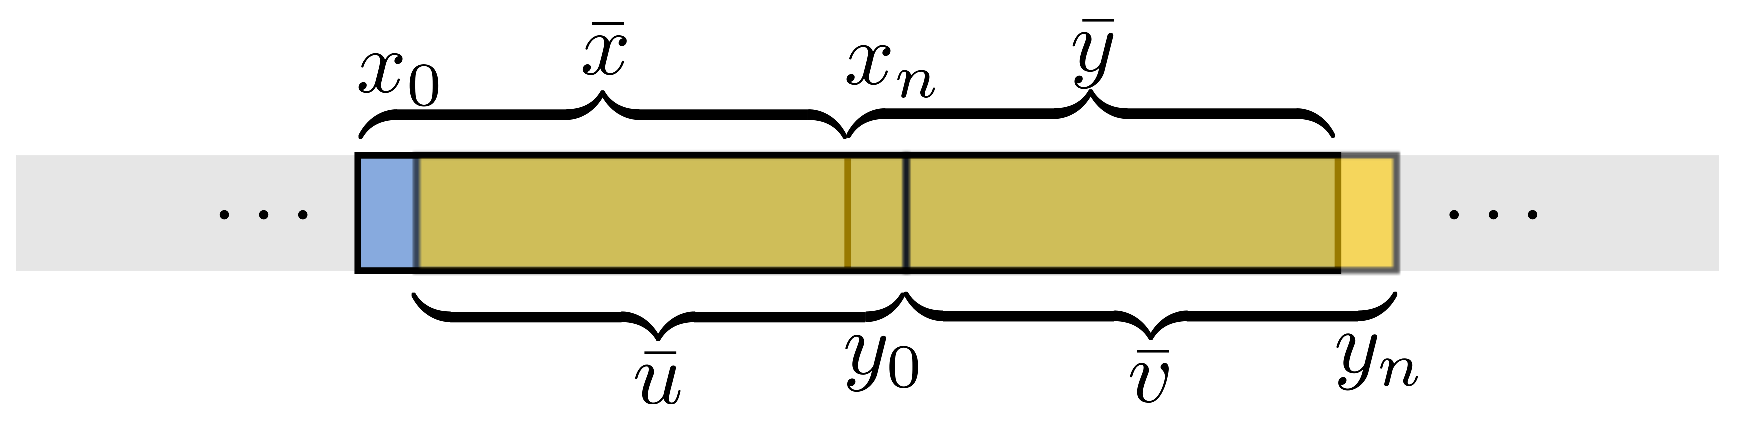
\includegraphics[width=0.8\textwidth]{correlation-windows-new}
	\caption{Correlation windows for the new update formulation}
	\label{fig:corr-win-new}
\end{figure}

As before, let $\{x_i\}_{i=0}^{n-1}$ and $\{y_i\}_{i=0}^{n-1}$ be complex
sequences corresponding to the symbols in the left window and the right window
respectively. Furthermore, let $\bar{x}$ and $\bar{y}$ be the means of the
left and right windows in the first time step. In the next time step, both
windows are moved one step to the right. Let the new means be $\bar{u}$ and
$\bar{v}$. This is shown diagrammatically in figure~\ref{fig:corr-win-new}.

Then we immediately have an update equation for the means themselves:
\begin{align}
	\bar{u} &= \bar{x} + \frac{x_n - x_0}{n} \\
	\bar{v} &= \bar{y} + \frac{y_n - x_0}{n}
\end{align}
We want to obtain $\sum_{i=1}^n{\corr{(x_i-\bar{u})}{(y_i-\bar{v})}}$ in terms
of $\sum_{i=0}^{n-1}{\corr{(x_i-\bar{x})}{(y_i-\bar{y})}}$.
\begin{equation}
	\begin{split}
		\sum_{i=1}^{n-1}{\corr{(x_i - \bar{x})}{(y_i - \bar{y})}}
		&= \sum_{i=1}^{n-1}{\corr{\left ( x_i - \bar{u} + \frac{x_n - x_0}{n} \right )}{\left ( y_i - \bar{v} + \frac{y_n-y_0}{n} \right )}} \\
		&= \sum_{i=1}^{n-1}{\corr{(x_i - \bar{u})}{(y_i - \bar{v})}} + \left ( \frac{x_n - x_0}{n} \right )\sum_{i=1}^{n-1}{(y_i - \bar{v})^*} \\
		& \quad + \left ( \frac{y_n - y_0}{n} \right )^*\sum_{i=1}^{n-1}{(x_i - \bar{u})} + \sum_{i=1}^{n-1}{\left ( \frac{x_n - x_0}{n} \right )\left ( \frac{y_n - y_0}{n} \right )^*}
	\end{split}
\end{equation}
Now,
\begin{align}
	\sum_{i=1}^{n-1}{(x_i - \bar{u})} &= \sum_{i=1}^{n-1}{x_i} - (n-1)\bar{u} \\
	                                  &= \sum_{i=1}^n{x_i}-x_n-(n-1)\bar{u} \\
	                                  &= n\bar{u} - x_n - (n-1)\bar{u} \\
	                                  &= \bar{u} - x_n
\end{align}
And similarly,
\begin{equation}
	\sum_{i=1}^{n-1}{(y_i - \bar{v})^*} = (\bar{v} - y_n)^*
\end{equation}
Therefore,
\begin{equation}
	\begin{split}
		\sum_{i=0}^{n-1}{\corr{(x_i - \bar{x})}{(y_i - \bar{y})}}
		&= \sum_{i=1}^n{\corr{(x_i - \bar{u})}{(y_i - \bar{v})}}
		   - \corr{(x_n - \bar{u})}{(y_n - \bar{v})} \\
		& \quad + \corr{(x_0 - \bar{x})}{(y_0 - \bar{y})}
		   + \left ( \frac{x_n - x_0}{n} \right )(\bar{v} - y_n)^* \\
		& \quad + \left ( \frac{y_n - y_0}{n} \right )^*(\bar{u} - x_n)
		   + (n-1) \left ( \frac{x_n - x_0}{n} \right ) \left ( \frac{y_n - y_0}{n} \right )^*
	\end{split}
\end{equation}
We can acquire the basic form of the update equation by rearranging terms:
\begin{equation} \label{eqn:new-update-0}
	\begin{split}
		c_{new} &= c_{old} - \left ( \frac{x_n - x_0}{n} \right ) (\bar{v} - y_n)^* - \left ( \frac{y_n - y_0}{n} \right )^* (\bar{u} - x_n) \\
		        & \quad - (n-1) \left ( \frac{x_n - x_0}{n} \right ) \left ( \frac{y_n - y_0}{n} \right )^* \\
		        & \quad + \corr{(x_n - \bar{u})}{(y_n - \bar{v})} - \corr{(x_0 - \bar{x})}{(y_0 - \bar{y})}
	\end{split}
\end{equation}

In order to simplify this expression to minimize the number of correlation terms, we need to group terms. If we group the $(n-1) \left ( \frac{x_n - x_0}{n} \right ) \left ( \frac{y_n - y_0}{n} \right )^*$ term with the $\left ( \frac{y_n - y_0}{n} \right )^* (\bar{u} - x_n)$ term, we get
\begin{equation}
	\begin{split}
		c_{new} &= c_{old} - \left ( \frac{x_n - x_0}{n} \right )(\bar{v} - y_n)^* \\
				& \quad - \left ( \frac{y_n - y_0}{n} \right )^* \left [ \bar{u} - x_n + \frac{n-1}{n}(x_n - x_0) \right ] \\
		        & \quad + \corr{(x_n - \bar{u})}{(y_n - \bar{v})} - \corr{(x_0 - \bar{x})}{(y_0 - \bar{y})}
	\end{split}
\end{equation}
Simplifying the $[\cdot]$ term,
\begin{equation}
	\begin{split}
		\frac{n\bar{u} - nx_n + (n-1)x_n - (n-1)x_0}{n} &= \frac{n\bar{u} - (n-1)x_0 - x_n}{n} \\
		                                                &= \frac{(n\bar{x} + x_n - x_0) - (n-1)x_0 - x_n}{n} \\
		                                                &= \bar{x} - x_0
	\end{split}
\end{equation}
So that
\begin{align}
	c_{new} &= c_{old} - \left ( \frac{x_n - x_0}{n} \right )(\bar{v} - y_n)^* - \left ( \frac{y_n - y_0}{n} \right )^*(\bar{x} - x_0) \notag \\
	        & \quad + \corr{(x_n - \bar{u})}{(y_n - \bar{v})} - \corr{(x_0 - \bar{x})}{(y_0 - \bar{y})} \notag \\
	        &= c_{old} + \corr{(\bar{u} - \bar{x})}{(y_n - \bar{v})} + \corr{(\bar{v} - \bar{y})}{(x_0 - \bar{x})} \notag \\
	        & \quad + \corr{(x_n - \bar{u})}{(y_n - \bar{v})} + \corr{(x_0 - \bar{x})}{(\bar{y} - y_0)} \notag \\
	        &= c_{old} + \corr{(\bar{u} - \bar{x} + x_n - \bar{u})}{(y_n - \bar{v})} \notag \\
	        & \quad + \corr{(x_0 - \bar{x})}{(\bar{v} - \bar{y} + \bar{y} - y_0)} \notag \\
	        &= c_{old} + \corr{(x_n - \bar{x})}{(y_n - \bar{v})} - \corr{(x_0 - \bar{x})}{(y_0 - \bar{v})} \label{eqn:new-update-1}
\end{align}

If instead we had grouped the $(n-1) \left ( \frac{x_n - x_0}{n} \right ) \left ( \frac{y_n - y_0}{n} \right )^*$ term with the $\left ( \frac{x_n - x_0}{n} \right )(\bar{v} - y_n)^*$ term, we would have arrived at the equivalent update equation
\begin{equation} \label{eqn:new-update-2}
	c_{new} = c_{old} + \corr{(x_n - \bar{u})}{(y_n - \bar{y})} - \corr{(x_0 - \bar{u})}{(y_0 - \bar{y})}
\end{equation}

Equations~\ref{eqn:new-update-1} and~\ref{eqn:new-update-2} together preserve
the inherent symmetry present in equation~\ref{eqn:new-update-0}. So even
though the individual equations seem to have lost the symmetry, it is still
preserved.

The same update equation can also be used for autocorrelation by setting
$x_i = y_i\;\forall\;i\in\{0,1,\ldots n-1\}$, $\bar{v} = \bar{u}$ and
$\bar{y} = \bar{x}$.

%%%%%%%%%%%%%%%%%%%%%%%%%%%%%%%%%%%%%%%%%%%%%%%%%%%%%%%%%%%%%%%%%%%%%%%%%%%%%%%

\section{Practical considerations}

\subsection{Cross-correlation cut-off for noisy regions}

We expect the absolute value of the cross-correlation of the two windows to be
much lower than the product of their autocorrelations. However, we found that
the value of the metric tended at times to be quite large, and even comparable
to the threshold used to determine the presence of a packet.

A possible reason for this might be the accumulation of errors due to the
running correlation algorithm being employed. In the regions of noise, both the
autocorrelation and cross-correlation values are low, however, random
fluctuations in the noise and in the error could sometimes cause them to become
roughly of the same order of magnitude.

In order to prevent erroneous packet detection in noisy regions, we introduced
a cut-off based on the absolute value of the cross-correlation. This cut-off
value must be empirically determined. If the absolute value of the
cross-correlation is less that the cut-off, we manually set the running
cross-correlation at the point to be zero, and skip all other checks for the
packet.

\begin{lstlisting}
	if(complex_abs(cross_corr) < CROSS_CORR_THRESHOLD) {
		cross_corr = Complex(0, 0);
		corr_coeff = 0;
	}
\end{lstlisting}

\subsection{Violation of Cauchy-Schwarz inequality}
\label{subsec:cs-violation}

We discovered that at certain instances, for example when searching for the
preamble towards the end of a previous frame, the value of the metric exceeded
unity. In a strict mathematical sense, this is impossible, since
cross-correlation is an inner product operation, and the Cauchy-Schwarz
inequality guarantees that
$$ \langle \ue{u}, \ue{v} \rangle \leqslant |\ue{u}||\ue{v}| $$
Nevertheless, the situation was observed. On closer inspection, we found that
at the edge of the frame, the values of the complex symbols dropped rapidly. In
such a situation, it took time for the cross-correlation value to settle (time
for the accumulated errors to diminish in comparison to the cross-correlation
value itself), whereas the autocorrelation values settled faster. This caused
the cross-correlation value to exceed the autocorrelation product, thus giving
a metric value greater than unity.

When checking for the preamble itself, we gave allowances for errors causing
the metric value to exceed unity. But in the situation described above, this
occurred with far larger deviations than we might expect due purely to floating
point error. In fact, the error was the accumulated error in the algorithm
itself. In such situations also, we manually set the cross-correlation value to
zero to avoid further propagation of this error.

\begin{lstlisting}
	abs1 = complex_abs(cross_corr);
	abs2 = sqrt(auto_corr_left * auto_corr_right);
	if(abs1 / abs2 > 1 + EPSILON) {
		// Violation of the Cauchy-Schwarz inequality!
		// Explicitly preserve it by killing the cross-correlation.
		abs1 = 0;
		corr_coeff = 0;
		cross_corr = Complex(0, 0);
	} else {
		corr_coeff = abs1 / abs2;
	}
\end{lstlisting}

\subsection{Fine metric}
\label{subsec:fine-metric}

When searching for the preamble in the body of a previous frame, we sometimes
found that the value of the metric exceeded the threshold. Essentially, the
values of the complex symbols within the frame depends on the data being
transmitted. It might so happen that the data produces a short repeating
pattern of the same length as the preamble in the bulk of the frame. In such a
situation, the timing synchronizer will erroneously detect a packet in the
middle of a frame.

This is because, so far, we have only correlated the first half of the preamble
with the second half in the received vector. We never correlated the received
symbols with the actual preamble values themselves (which are fixed, and thus
known at the receiver). It may not be possible to simply increase the threshold
until this stops happening, since the threshold value is determined by the
amount of noise in the system. %TODO: Insert ref to appendix with tuning.

To fix this issue, the fine metric is computed by correlating the first window
with the first half of the expected preamble. This is only done when the coarse
metric exceeds the threshold, since it is an expensive operation and since we
cannot use a running correlation algorithm to compute it. The fine metric value
has its own threshold, which is used as a second-pass for ensuring the presence
of an authentic preamble.

Note that even in the presence of an ISI channel, the fine metric will pick up
the most dominant channel tap. If $\ue{p}$ is the preamble vector and $\ue{h}$
is the channel, then the received preamble is
$$\ue{y} = \ue{p} * \ue{h}$$
This received vector is now correlated with the preamble itself, so that the
fine metric peaks at $\text{argmax}(\ue{h})$ with a peak value of
$\text{max}(\ue{h})$.

%TODO: Insert fine metric plot

\subsection{Going left for safety}
\label{subsec:safety}

In the event that the packet location as determined by the timing synchronizer
is not exactly correct, or in the event that there are several dominant taps
in the channel impulse response, we may not extract a good OFDM block. That is,
the OFDM block extracted may be polluted by the cyclic prefix of the subsequent
block. Such pollution cannot be corrected for by OFDM.

Therefore, to be \emph{safe}, we introduced a \verb+safety+ parameter. When
supplying the final packet location, we shift the packet \verb+safety+
positions to the left. This ensures that each OFDM block extracted will contain
only its own symbols. Instead of picking up symbols from the next block, we
would pick up symbols of the cyclic prefix of the same block. This can then be
corrected for by performing integer frequency offset estimation, in order to
rotate the block suitably. The final location of the packet that is returned is
therefore $$\texttt{packet\_loc} = \texttt{peak\_index} +
\texttt{preamble\_length} - \texttt{safety}$$

%%%%%%%%%%%%%%%%%%%%%%%%%%%%%%%%%%%%%%%%%%%%%%%%%%%%%%%%%%%%%%%%%%%%%%%%%%%%%%%

\section{Further optimizations}

On profiling the program, it was found that the timing synchronizer was the
slowest block, taking up to 50\% of the receiver program's run time. In order
to speed up the timing synchronizer to the extent possible, therefore, a few
more optimizations were performed that focused on reducing the amount of work
the timing synchronizer had to do.

\subsection{Stopping correlation after threshold breach}
\label{subsec:stop-corr}

The first optimization relies on the accuracy of the currently used timing
analysis algorithm. We found that the algorithm is quite selective in picking
out packets correctly. Given that this is the case, we assume that once the
fine metric threshold has been breached, a packet has been found, and that we
only need to find the dominant channel tap to find the best `location' of the
preamble.

Therefore, once the fine metric has been breached, we continue correlating only
up to a number \verb+max_time_steps_after_threshold+ of time steps. After this,
the point of maximum correlation is returned as the packet's location.

\subsection{Discarding the found frame block}
\label{subsec:frame-discard}

Once a preamble has been found in the two-frame block, we know that a full
frame follows. All symbols corresponding to this frame can then be removed from
the receive buffer so that we do not search what we know is part of a frame.

This way, we also (mostly) avoid the problems mentioned in
subsections~\ref{subsec:cs-violation} and~\ref{subsec:fine-metric}. Otherwise,
we would always have to scan the entirety of the second window, parts of which
might contain the frame body.\footnote{Note that we do not entirely avoid this
problem. In the presence of an ISI channel, the effective frame length is
longer than one \verb+frame_size+, and in the event that the preamble is found
at the end of the first window, it is possible that the frame edge goes outside
of the second frame window, meaning parts of the frame would be yet to be
received into the two-frame buffer. The other scenario where we may scan the
bulk of the frame in search of a packet is when the timing synchronizer fails
to detet a frame that is actually preset. In both these cases, we would
encounter symbols from the bulk of the frame, and thus the measures taken in
subsections~\ref{subsec:cs-violation} and~\ref{subsec:fine-metric} cannot be
done away with.}

We had remarked in subsection~\ref{subsec:two-frame-impl} that a one-frame
block is cumbersome and error-prone, since it is difficult to maintain and
update information on how many symbols have been extracted and how many more
are left to extract. Nevertheless, in the name of optimization, this is
exactly what we now proceed to do.

\begin{figure}[h]
	\centering
	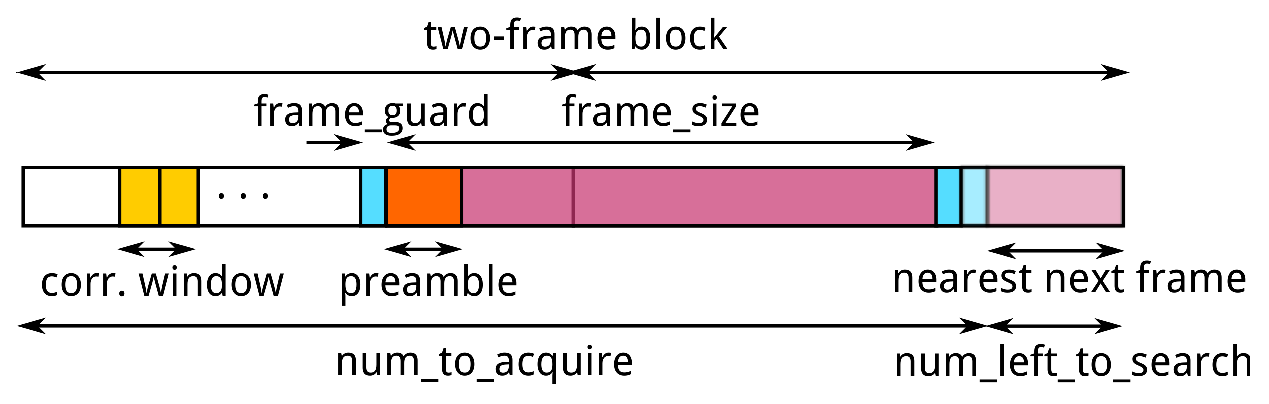
\includegraphics[width=0.8\textwidth]{two-frame-block-detailed}
	\caption{The two-frame block with \texttt{num\_to\_acquire} and
	         \texttt{num\_left\_to\_search} demarcated}
	\label{fig:two-frame-block-detailed}
\end{figure}

\begin{sloppypar}
We maintain two variables that describe the state of the two-frame block
\emph{outside} of the timing synchronizer at any given point in time. The first
is \texttt{num\_left\_to\_search}, which denotes the number of symbols that
are present in the two-frame block that have yet to be searched by the timing
synchronizer. The second is \verb+num_to_acquire+, which denotes the number of
symbols that have to be acquired from the complex data source in the current
iteration of the receive loop to fill the remainder of the buffer. While it is
redundant to maintain two variables, since we have
$\texttt{num\_left\_to\_search} + \texttt{num\_to\_acquire} = 2 \times
\texttt{frame\_size}$ but we do so for the sake of convenience.
\end{sloppypar}

During initialization, both \verb+num_to_acquire+ and \verb+num_left_to_search+
are set to \verb+frame_size+. When the first frame is found, it will be found
somewhere in the middle of the two-frame block. Let this point in the two-frame
block be \verb+packet_loc+. As mentioned in \ref{subsec:safety}, the packet
location returned is after the preamble, but then \verb+safety+ positions to
the left. Thus, from \verb+packet_loc+, we can discard $\texttt{frame\_size}
- \texttt{preamble\_length} + \texttt{safety}$ number of symbols.

To make sure that we do not read symbols at the end of the frame, we assume
that there is some minimum distance between two frames. This distance is called
the \verb+frame_guard+. The number of symbols to discard, from
\verb+packet_loc+ onwards, is then $\texttt{frame\_size}
- \texttt{preamble\_length} + \texttt{safety} + \texttt{frame\_guard}$. In
other words, the only relevant parameter, which is the number of symbols that
we still need to search through in the two-frame block is
\begin{equation}
	\begin{split}
		\texttt{num\_left\_to\_search} &= 2 \times \texttt{frame\_size} \\
		                               & \quad - (\texttt{frame\_size} - \texttt{preamble\_length} \\
		                               & \quad \quad \; + \texttt{safety} + \texttt{frame\_guard}) \\
		                               &= \texttt{frame\_size} + \texttt{preamble\_length} \\
		                               & \quad - \texttt{safety} - \texttt{frame\_guard}
	\end{split}
\end{equation}

\verb+num_to_acquire+, which is the number of symbols that need to be acquired
in the next iteration of the receive loop is then
$2 \times \texttt{frame\_size} - \texttt{num\_left\_to\_search}$.

\chapter{THE MODULARIZED OFDM STACK}
\label{chap:ofdm-stack}

%%%%%%%%%%%%%%%%%%%%%%%%%%%%%%%%%%%%%%%%%%%%%%%%%%%%%%%%%%%%%%%%%%%%%%%%%%%%%%%

\section{The goal}

Ideally, we wish to achieve a level of abstraction over the physical layer that
allows us to operate at the level of bit-streams. We would like to transmit the
bits with almost no knowledge of the underlying layer and mechanism. Suppose
bits were stored as arrays of \lstinline!char! elements, we would like to
transmit them with a single function call:

\begin{lstlisting}
	char *bits;
	// ... fill in the array
	transmit(bits);
\end{lstlisting}

Underlying this, there needs to be configurability. That is, if desired, we
should be able to break the abstraction and set options on the transmitter and
receiver. One way of doing this might be through a configuration file. But this
would mean that we cannot change parameters dynamically. So the underlying
framework should allow us to access internals in the code, if desired:

\begin{lstlisting}
	double freq = get_transmit_frequency();
	if(freq != 9e6) {        // Change freq to 900 MHz.
		change_transmit_frequency(9e6);
	}
\end{lstlisting}

In order to achieve this, we need to have a well-abstracted and modularized
code base. The data should be disconnected from the code to the maximum extent
possible. Different components of the code should be loosely coupled, that is,
there should be minimal interdependence between different modules, and they
should be maximally self-contained.

While, at present, the OFDM stack does not meet this ideal, one may at least
say that it has plotted itself a course and is well on its way.

%%%%%%%%%%%%%%%%%%%%%%%%%%%%%%%%%%%%%%%%%%%%%%%%%%%%%%%%%%%%%%%%%%%%%%%%%%%%%%%

\section{The modules}

The program has been functionally broken up into modules, as shown in
figure~\ref{fig:modules}.

%TODO: Figure showing modularity

A more detailed description of each of these modules follows.

\subsection{The mapper}

The mapper converts a sequence of bits into one of complex symbols. The reason
this has been kept outside of the OFDM framework is that different applications
have different requirements on the kinds of complex symbols generated.

Mapping may be performed on a coded bit stream, in which case it may be
sufficient to use a standard constellation to perform mapping. But in the
implementation of DPC, for example, we pre-subtract the expected interference
from another user. As a result, we do not transmit any fixed constellation
points. Any point in the available complex plane may be transmitted as a
symbol.

It is therefore best to allow for different kinds of mappers. In the interest
of keeping the OFDM framework loosely coupled with the mapping framework, the
two have been made into separate modules. The default mapper can now be
`unplugged' and a new, custom-defined mapper can be `plugged in' to the code.

\subsection{The OFDM Modulator}
\label{subsec:ofdm-modulator}

The OFDM Modulator converts a sequence of complex symbols into a sequence of
packets. Several configuration details come into play here, such as the number
of symbols that go into each frame, details of the preamble used in the frame,
etc.

In order to maintain a list of these values that can be used by the various
functions that fall under the ambit of the OFDM Modulator, the modulator has
been made into a class. The data members of the class allow for encapsulation
and abstraction, so that the settings are exposed for change only if desired.

A set of default parameters are automatically loaded when the object is
instantiated. Following this, settings can be changed by setting them manually
if desired. This can be done directly by assignment, since all data members are
public. After this, the object has to be initialized using the
\lstinline!initialize()! member function. This allocates memory and creates
\lstinline!fftw_plan!s. In a multi-threaded environment, this operation is not
thread-safe, and therefore must be completed before thread-creation.

In the transmit loop, the \lstinline!modulate()! call does the job of making
the symbols passed to it into packets. It returns a packet, which is a sequence
of time-domain complex symbols that can be transmitted using some sort of
transmitter.

\subsection{The USRP Transmitter}

The USRP Transmitter module is an encapsulated version of the UHD API for
transmission. As described in subsection~\ref{subsec:ofdm-modulator}, some
default parameters are loaded upon instantiation, which can be changed later.
Further, the \lstinline!add_options()! member function can be used to let the
module add its own set of options to the command line, via the
\lstinline!boost! \lstinline!program_options! module. All this must be
followed up with an \lstinline!initialize()! call.

The transmitter uses the \lstinline!transmit()! function to transmit symbols.
Usually, one packet of complex symbols (as received from the OFDM Modulator) is
transmitted at a time. However, there is really no such restriction. The
transmitter can be used independently of the OFDM modulator to transmit any
sequence of complex symbols.

\subsection{The USRP Receiver}

The USRP Receiver module is similar to the USRP Transmitter in all respects.
The \lstinline!receive()! call is used to receive a desired number of complex
symbols from the USRP.

\subsection{The OFDM Demodulator}

The OFDM Demodulator is the least independent of all the modules. It is also
the heaviest in terms of computational requirement and code size. The primary
reasons for the lack of its independence are the stringent requirements of the
timing analyser, given its working mechanism. It has a specific requirement on
the buffer size. Furthermore, in order to decrease the burden on the timing
analyser, we implemented frame-discarding, as described in
subsection~\ref{subsec:frame-discard}. This resulted in the use of the
unwieldy variables \lstinline!num_left_to_search! and
\lstinline!num_to_acquire!. These variables inevitably decrease the level of
independence of this module, because they force it to become coupled with the
process of acquisition of symbols (which is really different module's work), by
definition.

This module provides the \lstinline!demodulate()! member function to detect
whether or not packets are present in the given buffer, and if they are, then
to demodulate them and return a set of received complex symbols that should
have come from transmitted constellation points.

%%%%%%%%%%%%%%%%%%%%%%%%%%%%%%%%%%%%%%%%%%%%%%%%%%%%%%%%%%%%%%%%%%%%%%%%%%%%%%%

\section{Limitations}

While the modularized implementation has enabled plugging and unplugging of
various modules, there are still many things that this framework cannot do.

\subsection{Using two different kinds of frames}

It may sometimes be desirable to use two different kinds of frames, for eg.\ a
long data frame for transmitting information, and a short acknowledgement
frame, to tell the other side that a packet has been received. While the basic
structure is present for making use of two different kinds of frames, possibly
with different preambles or data masks, the implementation of the same is not
easy and requires some work on the part of the developer.

Currently, it is possible to create two or more different OfdmModulator and
OfdmDemodulator object pairs, and then manually specifying a different preamble
or data mask for each pair. Since all data members are public, they can be
directly changed after instantiation. An \lstinline!initialize()! call will
then allocate requisite memory, create \lstinline!fftw_plan!s and so on.

Modulation too, should not be a hassle. However, when calling the demodulate
function, there is some amount of coupling between the calling program and the
demodulator in the form of \lstinline!num_left_to_search! and
\lstinline!num_to_acquire!. If the \lstinline!frame_size!s of the two types
of frames are different, then during packet detection, we may get different
values of \lstinline!num_left_to_search! and \lstinline!num_to_acquire!
from each demodulator object. We would then have to create a temporary buffer
to manage the different requirements of \lstinline!num_left_to_search! and
\lstinline!num_to_acquire! for the two demodulators.

\subsection{Using single precision}

It is currently not possible to use single precision instead of double
precision, because the FFTW module in its present configuration uses only
double precision. While this by itself would not prevent us from using single
precision elsewhere, issues arise because at present, there are
\lstinline!reinterpret_cast!s between our flexible \lstinline!Complex! and
FFTW's less flexible \lstinline!fftw_complex! data types.

In order to use single precision everywhere, there is a need to refactor the
usage of FFTW, using preprocessor tricks to switch between
\lstinline!fftw_complex!, the double precision implementation and
\lstinline!fftwf_complex!, the single precision implementation, depending on
the value of a preprocessor variable.

\chapter{MODULES FOR DIRTY PAPER CODING}
\label{chap:dpc-modules}

The following are component modules in a larger framework that seeks to
implement Dirty Paper Coding \citep{Costa1983} real-time in the
case where a base station is transmitting to two users. The implementation
scheme for performing DPC is as explained in
\cite{ShilpaThangarajBhashyam2010}.

%%%%%%%%%%%%%%%%%%%%%%%%%%%%%%%%%%%%%%%%%%%%%%%%%%%%%%%%%%%%%%%%%%%%%%%%%%%%%%%

\section{Log Likelihood Ratio computation}

There is a requirement for the computation of log-likelihood ratios prior to
decoding the constellation symbols. Furthermore, this log-likelihood ratio is
to be computed on a repeated constellation.

The reason for this is that while transmitting symbols (from a base station to
a user in a 2-user system) in the DPC framework, interference from user 2 has
to be pre-subtracted from the constellation symbol being transmitted for user
1. During this process, it is possible that the symbol that is finally to be
transmitted lies outside of the constellation boundary. In such a situation,
the symbol in question is removed and reintroduced on the other side of the
constellation. The operation can be likened to a modulo operation, pulling
symbols outside of an interval back into the interval by repeatedly subtracting
the interval size.

On the receiver side, for the computation of LLRs, it is essential for
correctness to consider the possibility that a symbol might actually have come
from an out-of constellation point, or effectively from the other side of the
constellation. For the purpose of LLR computation, therefore, we can assume
that the symbol came from a repeated grid of the constellation.

This has currently been implemented only for a repeated 256-QAM constellation.

\subsection{Approximation of LLR}

The likelihood ratio is defined for each received bit as the ratio of the
probability of the corresponding transmitted bit being a 1 to to that of it
being a 0. This probability is computed for a given known noise variance, which
must be estimated beforehand.

In a 256-QAM constellation, the received constellation symbol could have come
from any of the 256 constellation points. Each constellation point encodes 8
bits. So from one received 256-QAM constellation point, we get 8 LLR values. At
any given bit position, half the constellation points will correspond to 0 and
the other half to 1. For computing the exact LLR value, we consider the
probability of the bit having come from each of these constellation symbols.

Let $s_i$ be the transmitted constellation points and $r$ be the received
complex vector. We wish to compute the LLR for a given bit (position) $b$. Let
$S^0$ be the set of indices $i$ for which $s_i$ has a 0 at bit position $b$,
and $S^1$ be the set of indices for which $s_i$ has a 1 at bit position $b$.
Then, the LLR for bit $b$ of the received vector $r$ is
\begin{equation}
	\text{LLR}(b) = \text{log} \left (
		\frac{ \sum_{i \in S^0}{e^{- |s_i - r|^2 / (2 \sigma^2)}} }
		     { \sum_{i \in S^1}{e^{- |s_i - r|^2 / (2 \sigma^2)}} }
		\right )
\end{equation}
where $\sigma^2$ is the noise variance.

To compute the LLR for each bit thus becomes very expensive, because it
involves 256 exponentiation operations. Since these LLR values are used only as
guides in the LDPC decoder, we do not need the exact LLR values. It is
sufficient to have good approximations of the same.

To this end, we neglect all terms except the dominant one in the numerator and
denominator of the likelihood ratio expression. That is to say, we redefine the
likelihood ratio as the ratio of the probability that the given received bit is
a 1, given that it came from the nearest constellation point having a 1 at the
corresponding bit location, to the probability that the given received bit is a
0, given that it came from the nearest constellation point having a 0 at the
corresponding bit location.
\begin{align}
	\text{LLR}_{\text{approx}}(b) &= \text{log} \left (
		\frac{ e^{- |s_{i^*_0} - r|^2 / (2 \sigma^2)} }
		     { e^{- |s_{i^*_1} - r|^2 / (2 \sigma^2)} }
		\right ) \\
		&= \frac{|s_{i^*_1} - r|^2 - |s_{i^*_0} - r|^2}{2 \sigma^2}
\end{align}
where $i^*_0$ corresponds to the nearest constellation point with index in
$S^0$ and $i^*_1$ corresponds to the nearest constellation point with index in
$S^1$.

\subsection{Computation of the approximate LLR}

In order to compute the approximate LLR for a bit, we need only the distance to
the constellation points corresponding to the nearest 0 and the nearest 1 for
that bit. To simplify our approach, we rely on the fact that \emph{the
constellation points corresponding to the nearest 0 and the nearest 1 are the
same (constant) for all points (all possible receive vectors) within the
decision region of each transmitted constellation point}.

In other words, we can precompute the constellation points corresponding to the
nearest 0 and the nearest 1 for each transmitted constellation point and store
these values in a table.  Then, we only need to find out the nearest
constellation point corresponding to a receive vector. This will tell us the
nearest 0 and the nearest 1 corresponding to a receive vector. Subtracting the
squares of the distances gives us the required LLR value.

\subsection{Nearest constellation point in a repeated constellation}

In order to compute the approximate LLR, we need to find the nearest
constellation point to the received vector. This is equivalent to the operation
of slicing, or locating which decision region the given receive vector lies
within. The only difference is that we need to do this in a repeated
constellation setting. This, in fact, makes our job a whole lot easier, because
it enables us to use floor and modulo operations.

\begin{figure}[h]
	\centering
	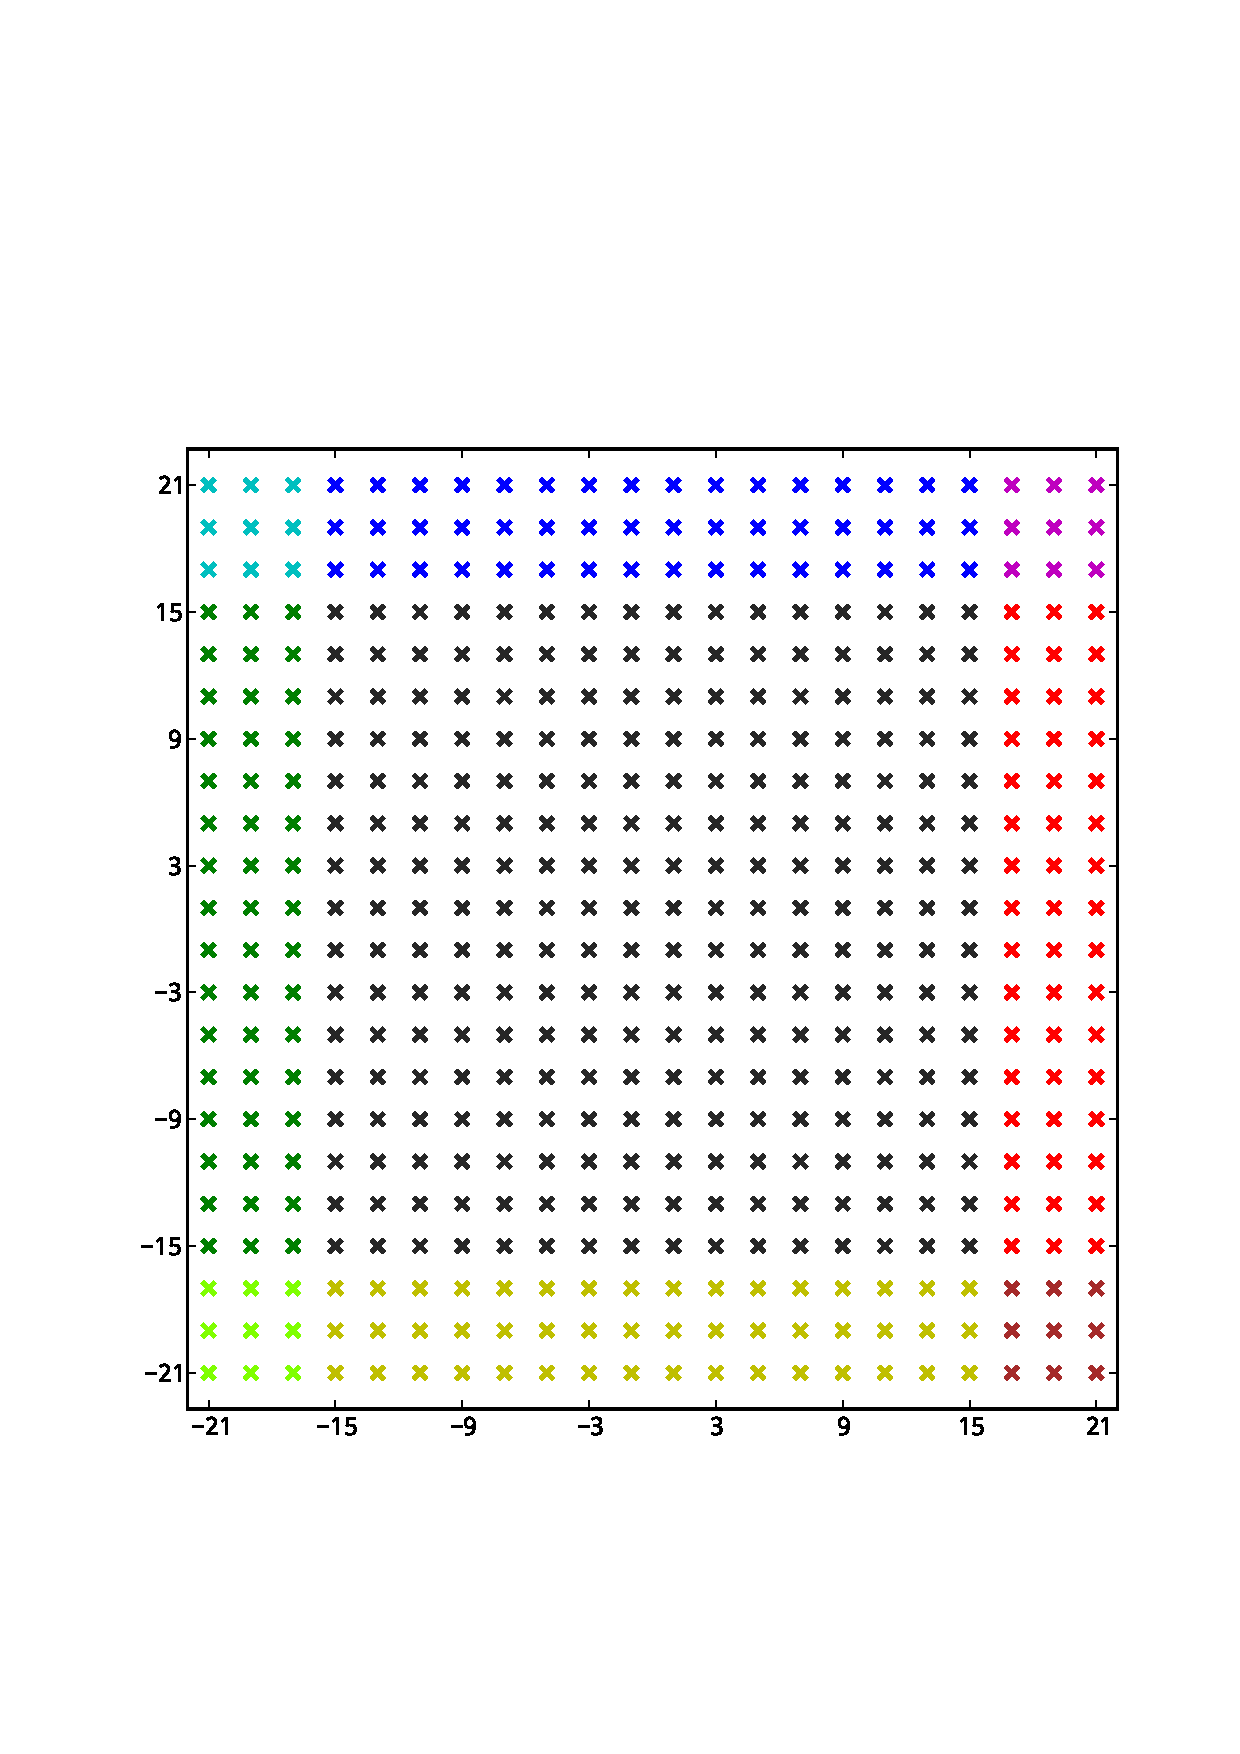
\includegraphics[width=0.8\textwidth]{256-qam-reptd-constln}
	\caption{Repeated 256-QAM constellation, prior to normalization. The
	         primary constellation is black, while its repetitions are coloured
	         variously.}
	\label{fig:256-qam-reptd}
\end{figure}

Consider the canonical 256-QAM constellation where constellation points are
located at odd points on the grid, from $-15$ to $+15$, on both real and
imaginary axes. On top of this, we have repetitions, so that the same
constellation is also present from $-47-15j$ to $-17+15j$ (left-bottom and
right-top corners of the constellation rectangle being used to denote
boundaries) on the left, from $-15+17j$ to $15+47j$ on the top, and so on in
all other directions (refer figure~\ref{fig:256-qam-reptd}).

Note that constellation points on $x=-17$ encode the same 8 bits as
constellation points on $x=+15$, and so on. This is the idea behind the
\emph{`modulo'} or the \emph{`repetition'}. This enables us to do the following
for slicing: we scale and translate the decision boundaries of the
constellation to the points of discontinuity of the floor function, and use the
floor function to achieve slicing. Following this, we use a modulo operation to
bring all repeated constellation points back into the primary constellation.

\begin{lstlisting}
	double x = creal(received_symbol);
	double y = cimag(received_symbol);
	// Move the received point back into the primary constellation
	x -= 32 * floor((x+16) / 32);
	y -= 32 * floor((y+16) / 32);
	// Find the index of the nearest constellation point
	int x_index = (int)(floor(x / 2) + 8);
	int y_index = (int)(floor(y / 2) + 8);
\end{lstlisting}

%%%%%%%%%%%%%%%%%%%%%%%%%%%%%%%%%%%%%%%%%%%%%%%%%%%%%%%%%%%%%%%%%%%%%%%%%%%%%%%

\section{Viterbi algorithm for Joint Trellis Shaping}

Joint Trellis shaping is aimed at minimizing the transmitted constellation
energy over a large number of constellation symbols. In order to do this with
greater ease, we use an almost-Gray mapping scheme for the constellation.

The mapping for 256-QAM is based off the mapping for 16-PAM. The first four
bits are mapped using a 16-PAM constellation to get the real part of the
256-QAM constellation point. Similarly, the next four bits are used to get the
imaginary part.

\begin{figure}[h]
	\centering
	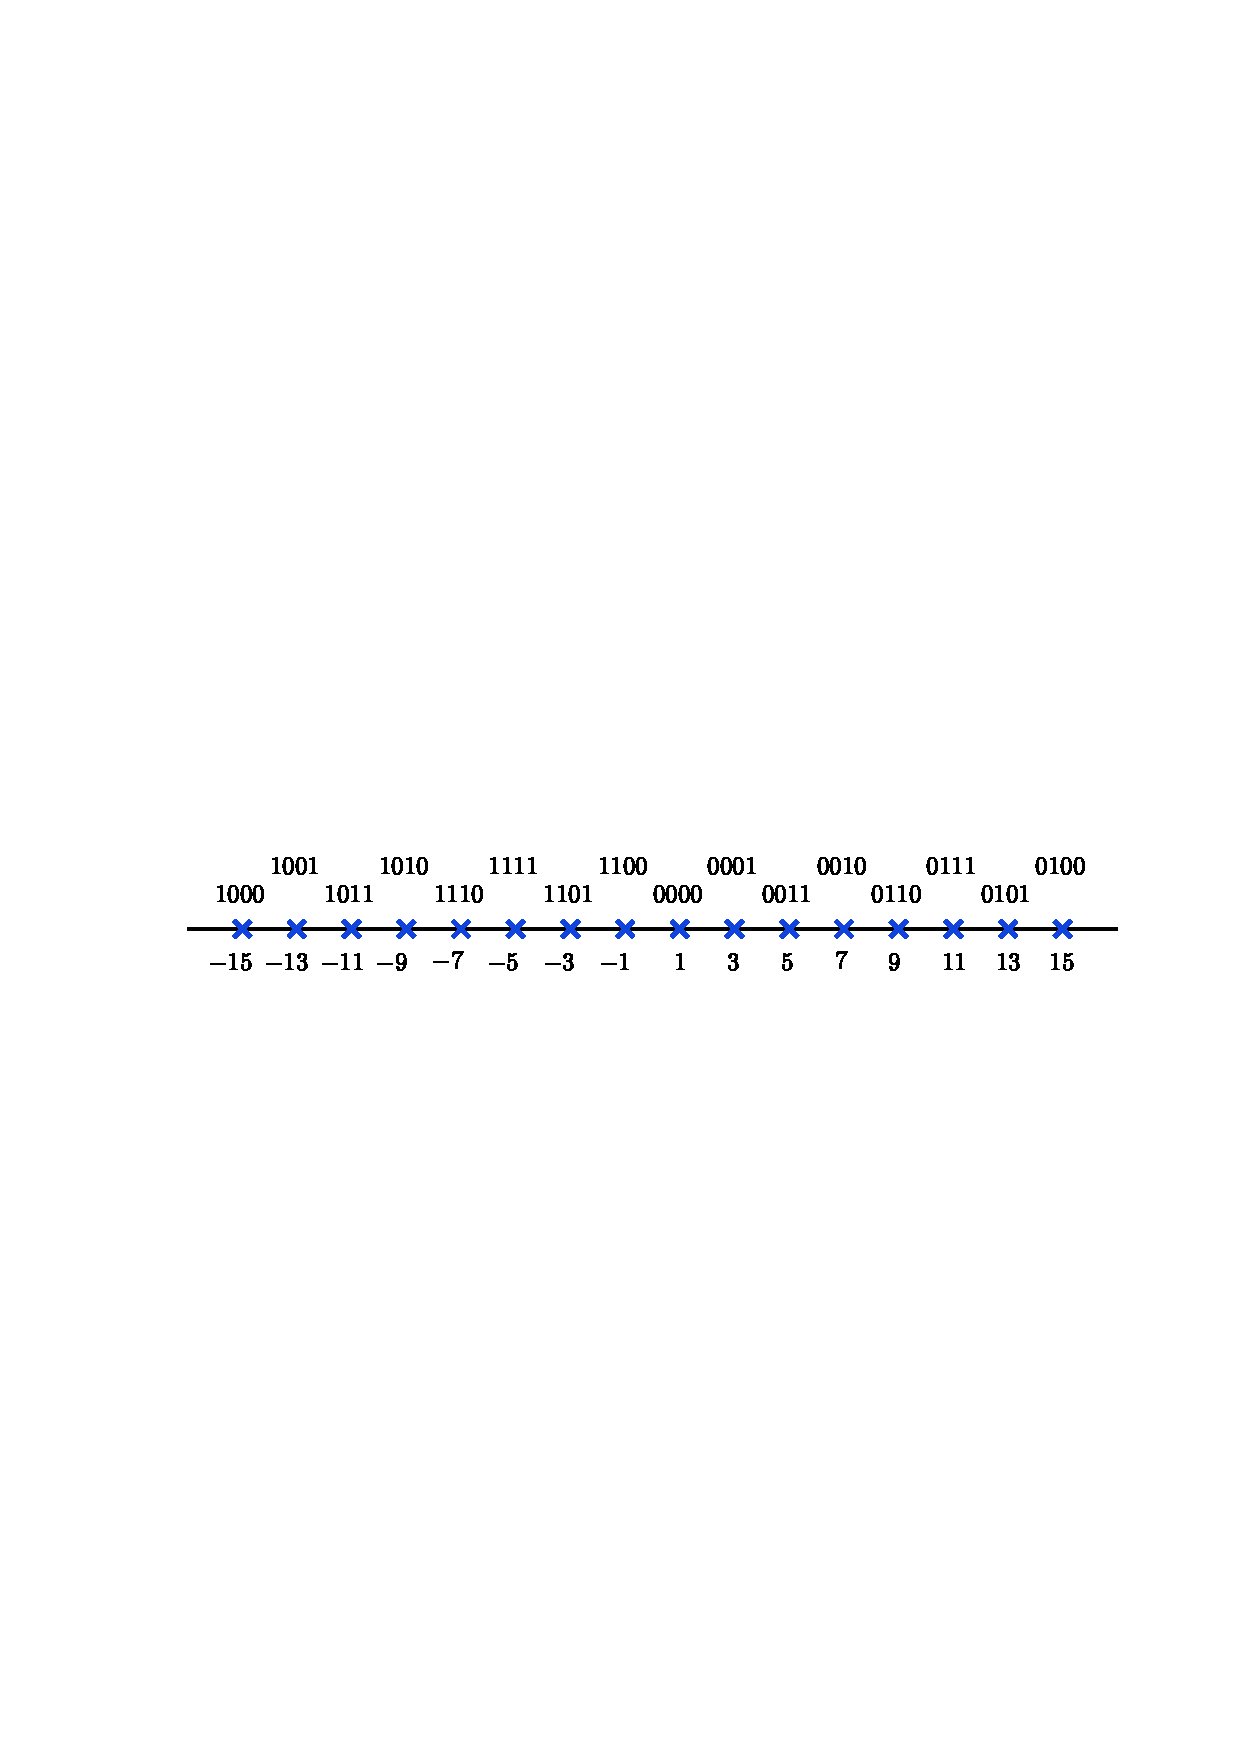
\includegraphics[width=\textwidth]{16-pam-constln}
	\caption{16-PAM constellation with mapping shown}
	\label{fig:16-pam}
\end{figure}

The 16-PAM constellation used is almost-Gray coded, as shown in
figure~\ref{fig:16-pam}. Notice that the last three bits read the same when
starting at $-15$ and going right, and when starting at $+1$ and going right.
The first bit, i.e.\ the sign bit, can therefore be used to position the
constellation point towards the centre of the constellation (with lower energy)
or towards the edge of the constellation (with higher energy).

The point of trellis shaping is to choose sign bits in such a way as to
minimize the overall constellation energy, averaged over many transmitted
symbols. In the case of DPC, we need to perform joint trellis shaping, wherein
we minimize the overall average constellation energy of two users. To achieve
this the optimal way, we make use of the Viterbi algorithm.

\subsection{Shaping using the trellis}

The Viterbi algorithm \citep{Viterbi1967} is used to find the optimal sequence
of signed bits to minimize the overall energy of the transmitted symbols.
Different choices of signed bits make different paths in the trellis. The
branch metric corresponds to the energy of the constellation point generated by
a certain choice of sign bits. Thus, by finding the optimal path, we minimize
the overall transmit energy.

\subsection{Implementing the Viterbi algorithm}

In the Viterbi algorithm, edge weights (or the branch metrics) denote the
`cost' of choosing a certain path and node weights denote the accumulated
minimum cost of reaching that particular node.

We start by assigning a node weight of zero to the left-most states in the
trellis. Following this, at `time step', we need to compute the edge weights.
Given a set of input bits, we need to evaluate all possible choices of sign
bits. Each edge's weight is then the transmitted energy of the corresponding
constellation point that results from choosing that particular sign bit. Next,
we need to update the node weights of the next time step. This is done by
choosing, for each node, an input edge, which yields the least cost after
adding its branch metric with the corresponding source node's weight. A summary
of this algorithm in pseudocode is presented in algorithm~\ref{alg:viterbi}.

\begin{algorithm}[h]
	\SetKwData{Edge}{edge} \SetKwData{ToNode}{to\_node} \SetKwData{FromNode}{from\_node} \SetKwData{StateDiagram}{state\_diagram} \SetKwData{Weight}{weight}
	\SetKwData{MinNode}{min\_node} \SetKwData{PrevNode}{prev\_node} \SetKwData{Path}{path} \SetKwData{Node}{node}
	\SetKwFunction{Min}{Min} \SetKwFunction{Compute}{Compute}
	\SetKwInOut{Input}{input} \SetKwInOut{Output}{output}

	\Input{\StateDiagram;$\;$\emph{input bits for \Edge.\Weight computation}}
	\Output{\Path}
	\BlankLine
	\emph{initialize start node weights to $0$}\;
	\emph{initialize all other node weights to $\infty$}\;
	\ForAll{time steps} {
		\ForEach{\Edge in \StateDiagram} {
			\Compute{\Edge.\Weight}\;
			\If{\Edge.\ToNode.\Weight $>$ \Edge.\FromNode.\Weight $+$ \Edge.\Weight} {
				\Edge.\ToNode.\Weight $\leftarrow$ \Edge.\FromNode.\Weight $+$ \Edge.\Weight\;
				\Edge.\ToNode.\PrevNode $\leftarrow$ \Edge.\FromNode\;
			}
		}
	}
	\MinNode $\leftarrow$ \Min{final nodes}\;
	\Node $\leftarrow$ \MinNode\;
	\While{\Node not in start nodes} {
		\Path $\leftarrow$ \Node\;
		\Node $\leftarrow$ \Node.\PrevNode\;
	}
	\Return \Path\;
	\caption{The Viterbi algorithm}
	\label{alg:viterbi}
\end{algorithm}


%%%%%%%%%%%%%%%%%%%%%%%%%%%%%%%%%%%%%%%%%%%%%%%%%%%%%%%%%%%%%%%%%%%%%%%%%%%%%%%
% Appendices

\appendix

\chapter{APPENDIX}

%%%%%%%%%%%%%%%%%%%%%%%%%%%%%%%%%%%%%%%%%%%%%%%%%%%%%%%%%%%%%%%%%%%%%%%%%%%%%%%
% Bibliography

\begin{singlespace}
  \bibliography{refs}
\end{singlespace}

\end{document}
